\makesection{Physics}

\begin{frame}{Decoupling Frame Rate and Physics}
    \vspace{-0.25cm}
    \includegraphics<1>[width=\textwidth]{figures/ploop/1.pdf}
    \includegraphics<2>[width=\textwidth]{figures/ploop/2.pdf}
    \includegraphics<3>[width=\textwidth]{figures/ploop/3.pdf}
    \includegraphics<4>[width=\textwidth]{figures/ploop/4.pdf}
    \includegraphics<5>[width=\textwidth]{figures/ploop/5.pdf}
    \includegraphics<6>[width=\textwidth]{figures/ploop/6.pdf}
    \includegraphics<7>[width=\textwidth]{figures/ploop/7.pdf}
    \includegraphics<8>[width=\textwidth]{figures/ploop/8.pdf}
    %\includegraphics<9>[width=\textwidth]{figures/ploop/9.pdf}

    \onslide<8>{
        \vspace{-1.1cm}
        \begin{flushright}
            \footnotesize(Fiedler \cite{gafferTimestep})
        \end{flushright}
    }
\end{frame}

\begin{frame}{The Physics Update}
    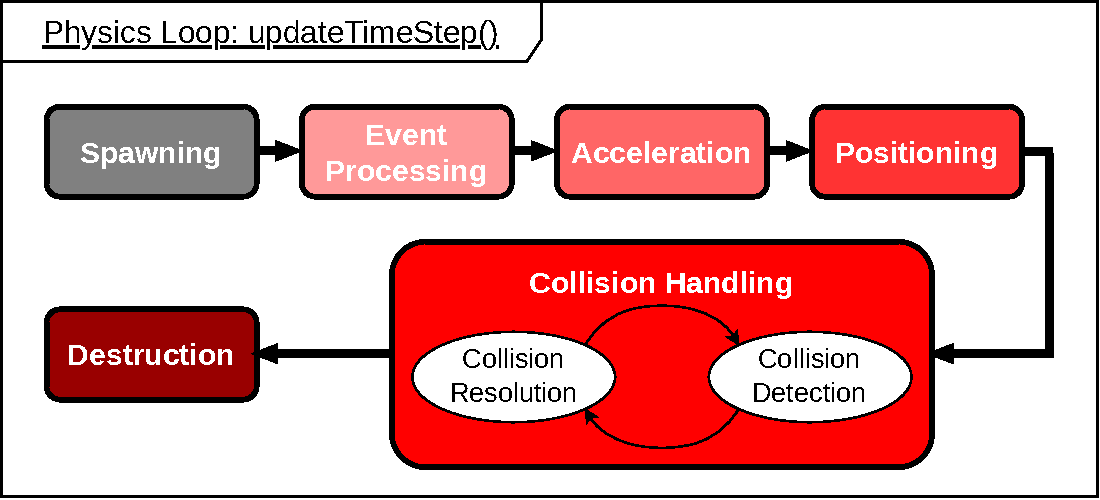
\includegraphics[width=\textwidth]{../figures/physics/updateTimeStep.pdf}
\end{frame}

%\begin{frame}{Colliding Entities}
%    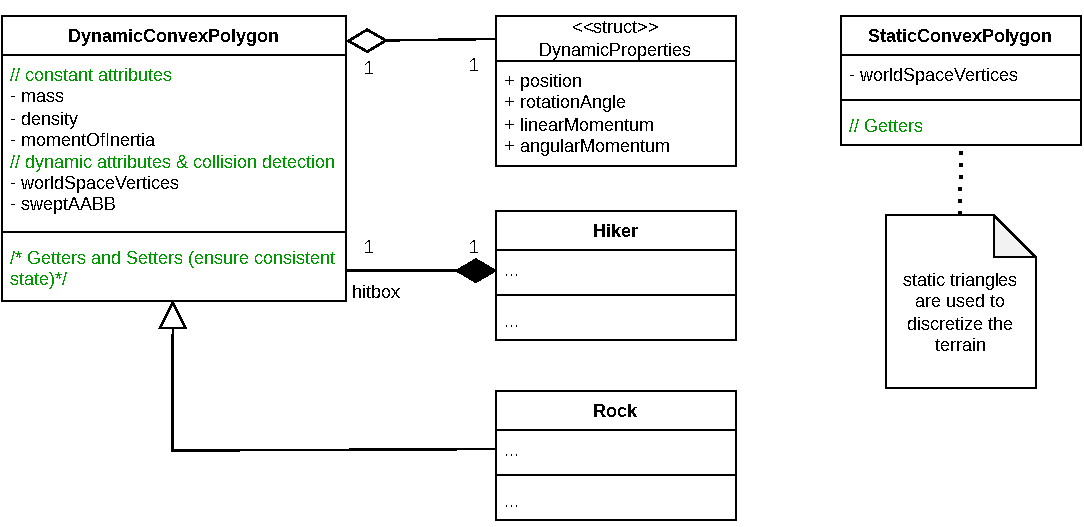
\includegraphics[width=\textwidth]{../figures/physics/rockStateUML3.pdf}
%\end{frame}

\begin{frame}{Movement Equations}
    \begin{itemize}
        \item Based on forces and impulses instead of velocities \cite{baraff}.
        \item Simulated entities have linear and angular momentum.
        \item Movement is governed by:
        \begin{itemize}
            \item Gravitational force (body force)
            \item Collision impulses (surface impulses)
        \end{itemize}
        \item System of continuous ODEs is discretized with the symplectic euler method.
    \end{itemize}
    \begin{minipage}{\textwidth}
        \centering
        \begin{minipage}{.495\textwidth}
            \begin{align*}
                \frac{\textbf{d}}{\textbf{d}{t}} 
                \left(
                  \begin{array}{c}
                    \overrightarrow{x}(t)\\
                    \overrightarrow{P}(t)\\
                    \theta(t)\\
                    L(t)
                  \end{array}
                \right)
                =
                \left(
                  \begin{array}{c}
                    {\overrightarrow{P}(t)}/{m}\\
                    \overrightarrow{F}(t)\\
                    L(t)/I\\
                    \tau(t)
                  \end{array}
                \right)
            \end{align*}
        \end{minipage}
        \begin{minipage}{.495\textwidth}
            \begin{align*}
                \overrightarrow{P}^{t+1} &= \overrightarrow{P}^{t} + \delta t \cdot \overrightarrow{F}^{t}\\
                \overrightarrow{x}^{t+1} &= \overrightarrow{x}^{t} + \delta t \cdot \frac{\overrightarrow{P}^{t+1}}{m}\\
                L^{t+1} &= L^{t} + \delta t \cdot \tau^{t}\\
                \theta^{t+1} &= \theta^{t} + \delta t \cdot \frac{L^{t+1}}{I}
              \end{align*}
        \end{minipage}
    \end{minipage}
\end{frame}

\begin{frame}{Collision Detection: Broadphase (swept AABBs \cite{sweptAABB})}
  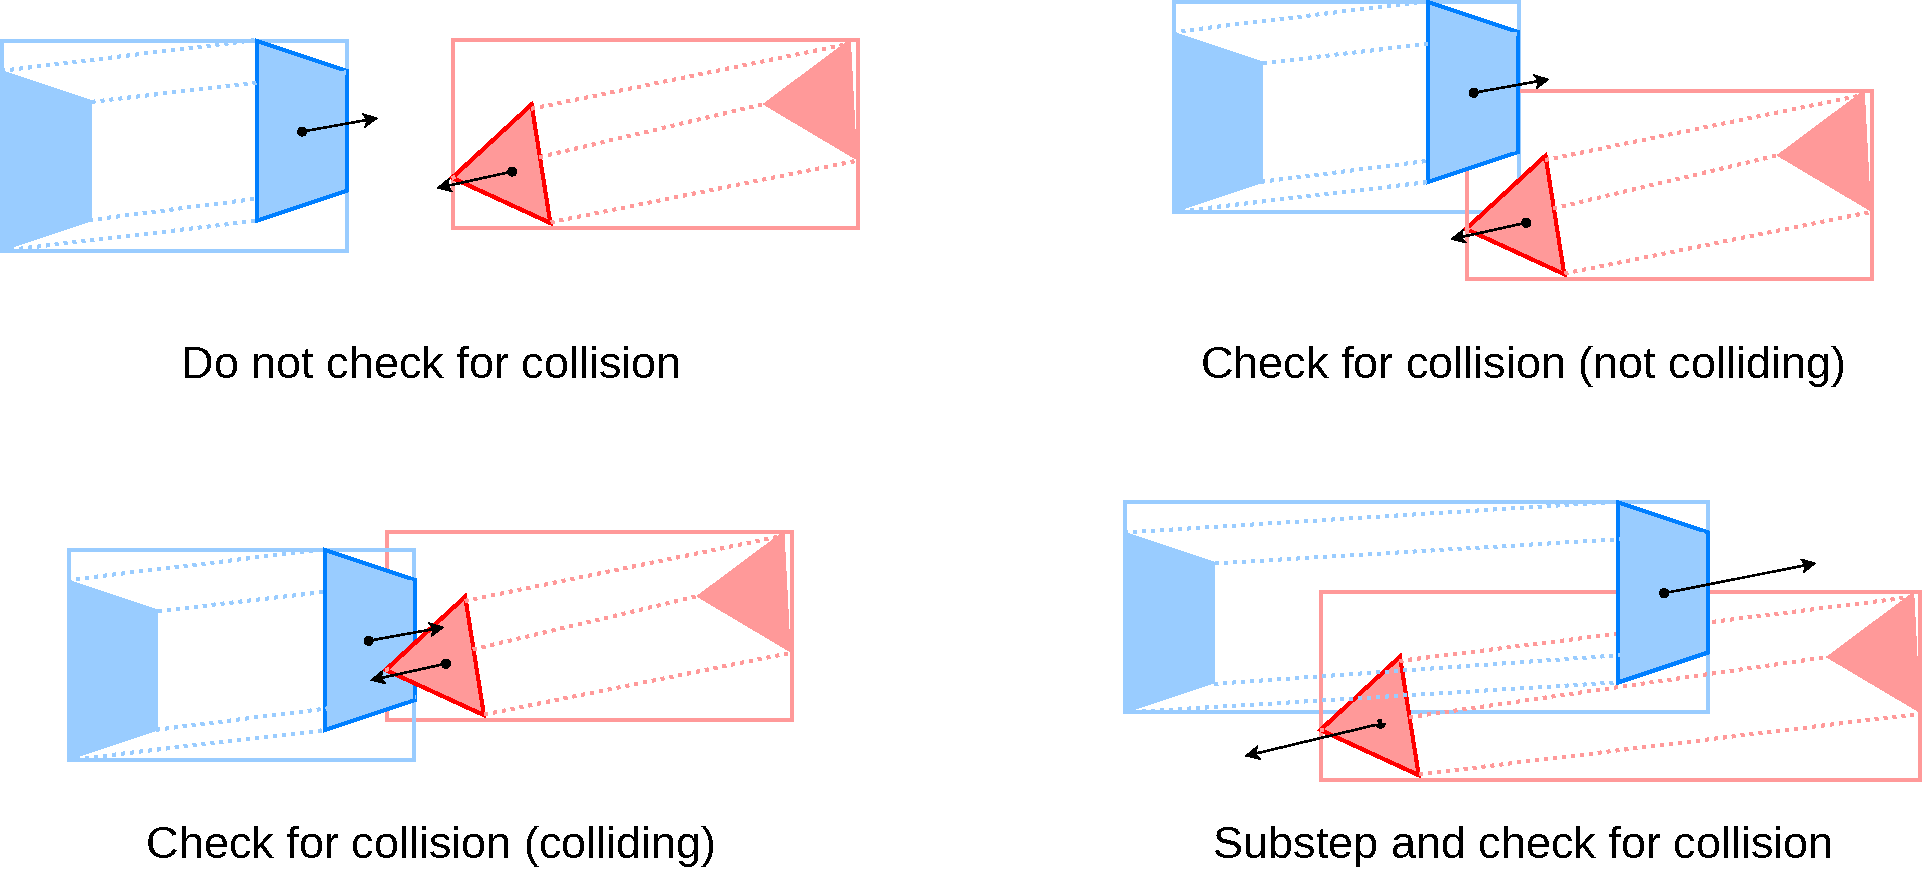
\includegraphics[width = \textwidth]{../figures/physics/aabb_extended.pdf}
\end{frame}

\begin{frame}{Collision Detection: Narrowphase (SAT \cite{geometrySAT})}
    \centering
    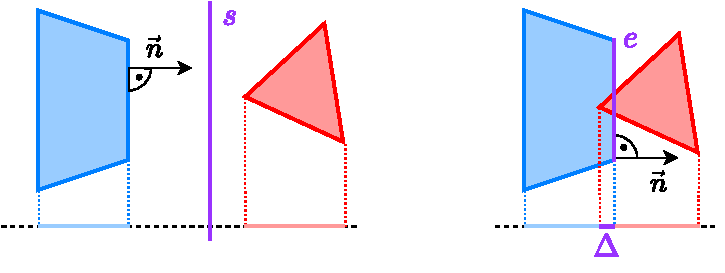
\includegraphics[width = \textwidth]{../figures/physics/sat2.pdf}
\end{frame}

\begin{frame}{Collision Resolution}
    \begin{figure}
        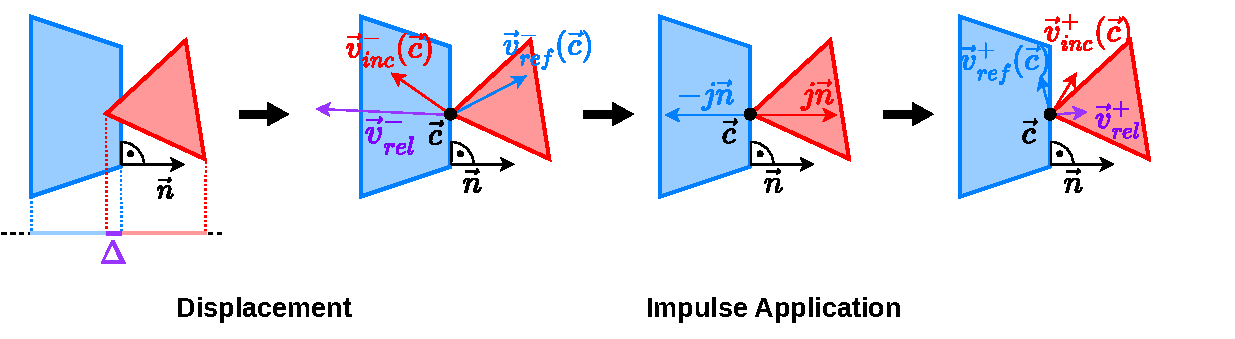
\includegraphics[width = \textwidth]{../figures/physics/resolution2.pdf}
    \end{figure}
    \begin{itemize}
        \item Empirical Law for Frictionless Collisions \cite{baraff}: $\left<\overrightarrow{v}_{rel}^{\,+}, \overrightarrow{n}\right> = -\epsilon\left<\overrightarrow{v}_{rel}^{\,-}, \overrightarrow{n}\right>$
        \item $\epsilon$ is the coefficient of restitution (``bounciness factor'')
    \end{itemize}
\end{frame}

\begin{frame}{Types of Collisions}
    \begin{minipage}{\textwidth}
        \centering
        \begin{minipage}{0.24\textwidth}
            \centering
            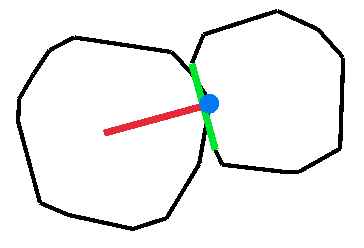
\includegraphics[width=\textwidth]{figures/colls/rrw.png}
        \end{minipage}
        \begin{minipage}{0.24\textwidth}
            \centering
            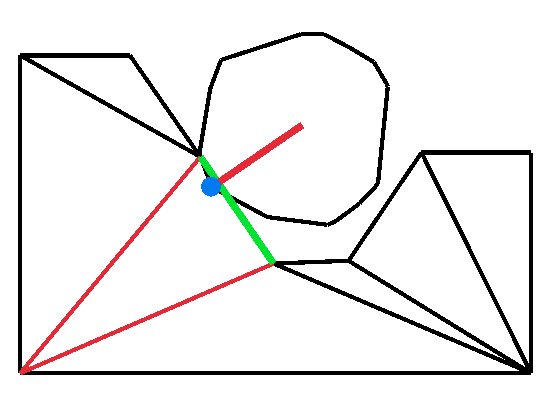
\includegraphics[width=\textwidth]{figures/colls/rtw.png}
        \end{minipage}
        \begin{minipage}{0.24\textwidth}
            \centering
            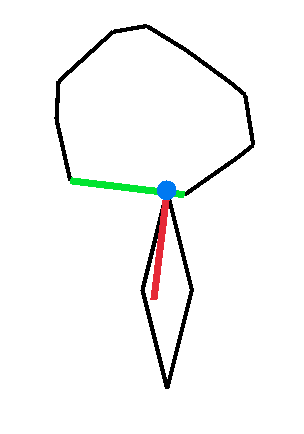
\includegraphics[width=.8\textwidth]{figures/colls/rhw.png}
        \end{minipage}
        \begin{minipage}{0.24\textwidth}
            \centering
            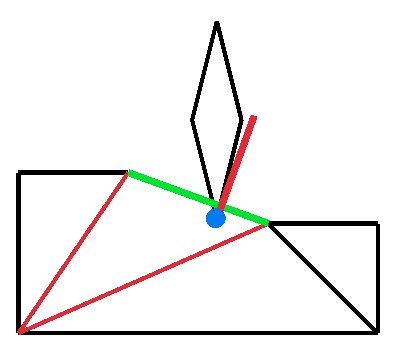
\includegraphics[width=\textwidth]{figures/colls/htw.png}
        \end{minipage}
    \end{minipage}
    \begin{minipage}{\textwidth}
        \centering
        \begin{minipage}{0.24\textwidth}
            \centering
            Rock-Rock
        \end{minipage}
        \begin{minipage}{0.24\textwidth}
            \centering
            Rock-Terrain
        \end{minipage}
        \begin{minipage}{0.24\textwidth}
            \centering
            Rock-Hiker
        \end{minipage}
        \begin{minipage}{0.24\textwidth}
            \centering
            Hiker-Terrain
        \end{minipage}
    \end{minipage}
\end{frame}

%\begin{frame}{Performance Considerations}
%    \begin{itemize}
%        \item Performance optimizations for handling large numbers of entities.
%        \item Usage of swept AABBs prunes collision checks with SAT.
%        \item Warm starting to further reduce cost of the SAT algorithm.
%        \item Pre-computation of world-space coordinates and AABBs upon moving an entity instead of during every collision check.
%        \item Effective garbage collection for entities and terrain that leave the scope of the game.
%    \end{itemize}
%    \centering
%    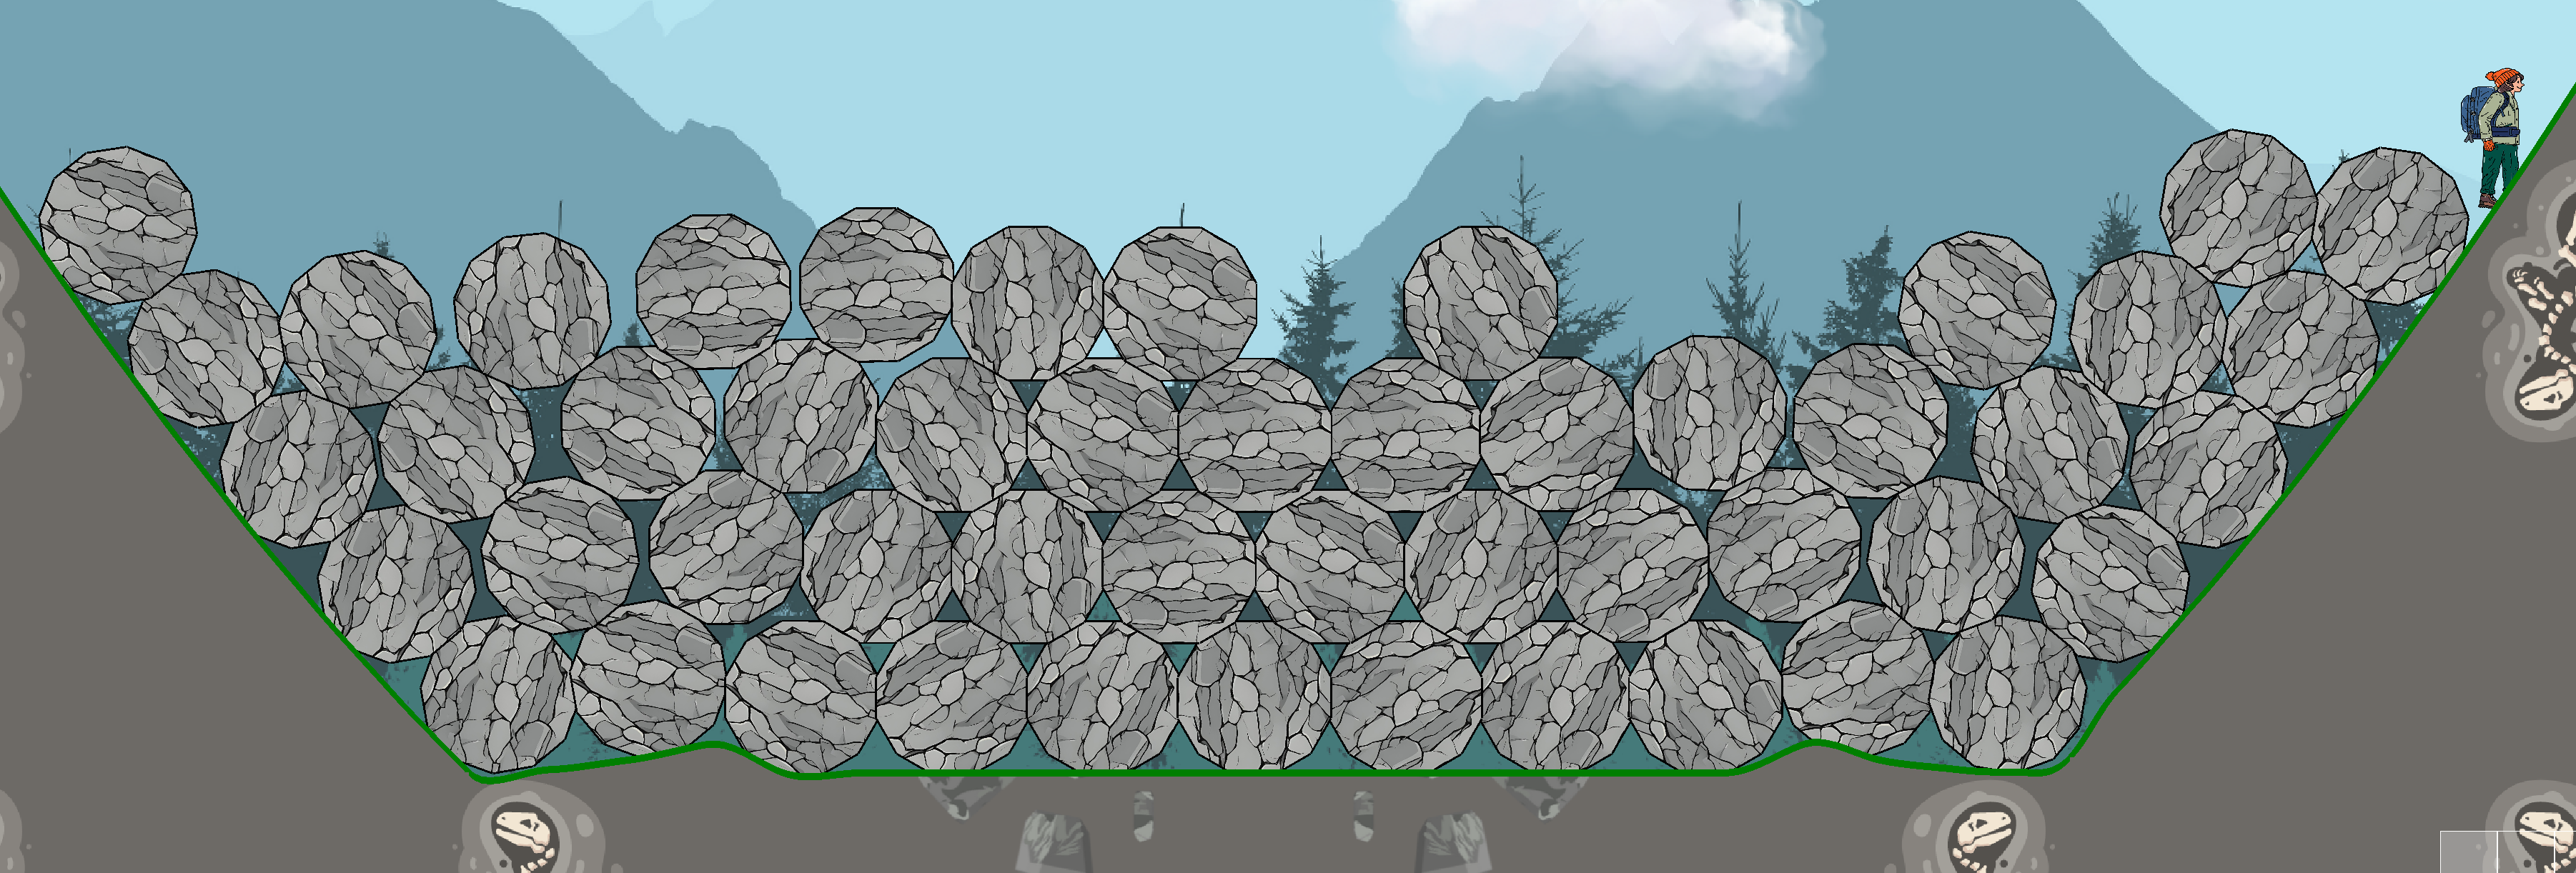
\includegraphics[width=.6\textwidth]{figures/sim.png}
%\end{frame}